% 02-methods.tex

% Section Title
\section{METHODS} \label{sec:methods}

    % In prose, describe the end-to-end procedure
    % - Devices and software: handset model, app, toolbox X
    % - Data collection: where, how long, static vs. moving X
    % - Spoofed-inputs: false position and delay parameters
    % - Optional interference scenario
    % - Processing: filtering criteria and solver workflow X

    \subsection{Devices and Software}
    
        We used a Samsung Galaxy A51 with Android 11 for this experiment.
        GNSS Logger v3.1.0.4 was chosen due to its unrestricted access to raw GNSS measurements, compatibility with newer Android APIs, and ability to record detailed GNSS data that is suitable for precise analysis.
        MATLAB R2024b was employed to handle data because it comes with Google's GNSS toolbox, which accommodates robust analysis and visualization of GNSS measurements and position solutions.
        
    \subsection{Data Collection Procedure}
    
        Two distinct 5-minute GNSS data logging sessions were conducted on 3 May 2025, under cloudy weather conditions, using the GNSS Logger app configured with the following settings enabled:

        \begin{itemize}
            \item \textbf{GNSS Location:} Enabled to capture location data.
            \item \textbf{GNSS Measurements:} Enabled to log raw GNSS measurements.
            \item \textbf{Navigation Messages:} Enabled to capture navigation data.
            \item \textbf{GnssStatus:} Enabled to log GNSS status information.
            \item \textbf{Sensors:} Enabled to capture sensor data.
        \end{itemize}
        
        The sessions were designed to capture both static and dynamic GNSS performance, with the following details:

        \begin{itemize}
            \item \textbf{Static Scenario:} Performed on the rooftop of Monte dei Cappuccini, Turin, starting at 10:35:20. The device was stationary throughout the entire session, providing baseline measurements.
            \item \textbf{Dynamic Scenario:} Conducted on tram line 15 from Piazza Castello to Piazza Vittorio Veneto, starting at 10:00:21, simulating a typical urban mobility scenario.
        \end{itemize}

        \begin{figure}[h!]
          \centering
          \begin{subfigure}{0.23\textwidth}
              \centering
              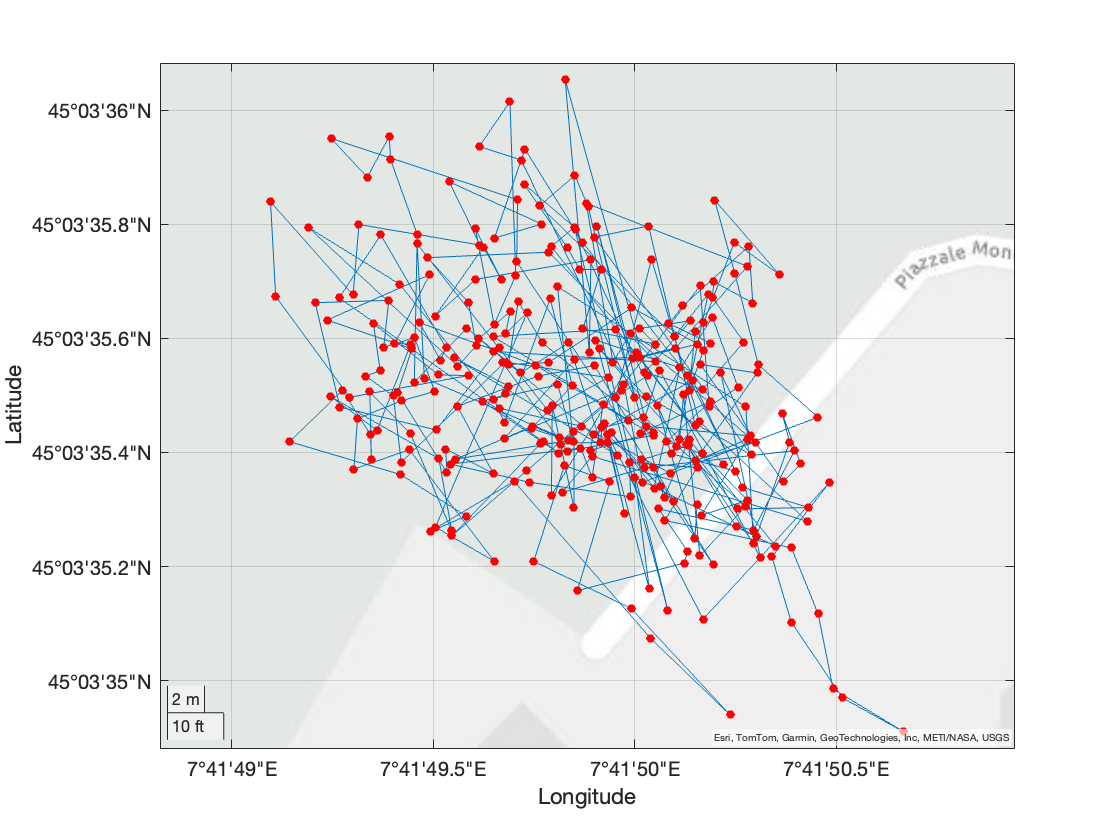
\includegraphics[width=\textwidth]{images/Monte_Cappuccini/filtered/Samsung_A51_Monte_Cappuccini_fig6.png}
              \caption{Monte dei Cappuccini.}
              \label{fig:static_scenario}
          \end{subfigure}
          \hfill
          \begin{subfigure}{0.23\textwidth}
              \centering
              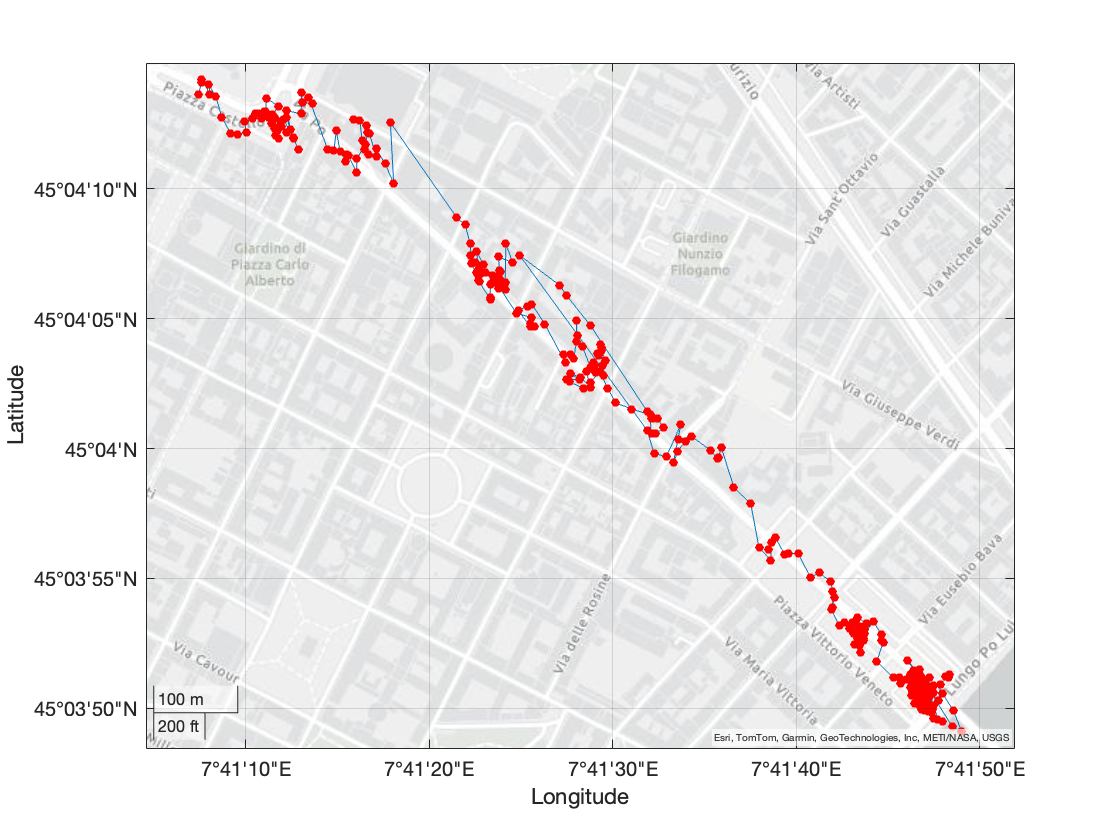
\includegraphics[width=\textwidth]{images/Tram_15_trip_Castello_to_Pescatore/filtered/Samsung_A51_Tram_15_trip_Castello_to_Pescatore_fig6.png}
              \caption{Tram Line 15.}
              \label{fig:dynamic_scenario}
          \end{subfigure}
          \vspace{0.35cm}
          \caption{Comparison of GNSS data: (a) Static scenario at Monte dei Cappuccini,(b) dynamic scenario along Tram Line 15.}
          \label{fig:gnss_comparison}
        \end{figure}

    \subsection{Processing Pipeline}
    
        The raw GNSS data from the GNSS Logger served as the input dataset for MATLAB. 
        Processing involved a scripted workflow via \cooltext{ProcessGnssMeasScript.m}, where the following steps were executed:
        
        \begin{enumerate}
            \item \textbf{Filtering:} Data points with a carrier-to-noise ratio below 25 dB-Hz or satellite elevations below 15° were excluded to improve accuracy.
            \item \textbf{Measurement Extraction:} Pseudorange and Doppler measurements were computed from GNSS timestamps and satellite transmission data.
            \item \textbf{Weighted Least Squares (WLS) Positioning:} Applied to derive precise positioning and clock bias estimates.
            \item \textbf{Visualization and Comparison:} Output plots from MATLAB, including pseudorange, pseudorange rates, and position solutions, were generated to facilitate comparative analysis of the static and dynamic scenarios.
        \end{enumerate}

        Results from this processing pipeline provided insights into the differences in GNSS performance under static and dynamic conditions.
    
    \subsection{Spoofed-Input Configuration}

        Spoofing scenarios were emulated by introducing artificial variations to the recorded GNSS data through MATLAB processing. 
        Specifically, mock positions were assigned by adjusting the parameter \cooltext{spoof.position}, which represents modified latitude, longitude, and altitude coordinates. 
        Additionally, artificial time delays were tested by adjusting the \cooltext{spoof.delay} parameter, typically in milliseconds, to mimic delayed GNSS signal arrival. 
        Such configurations facilitated evaluation of the impact of spoofing scenarios on position estimation reliability and accuracy.

    \subsection{Optional Interference Scenario}
    
        Even a worst-case interference situation was simulated, replicating conditions in the vicinity of potential interference sources such as broadcasting antennas or communication areas of high density. 
        GNSS data were collected near such sources of interference, and then processed with the same MATLAB procedure. 
        Nominal condition comparison was established to analyze the impact of external interference on GNSS observables such as variation in pseudorange measurements, carrier-to-noise ratio, and positional accuracy overall.
